%%
%% Automatically generated file from DocOnce source
%% (https://github.com/hplgit/doconce/)
%%
%%
% #ifdef PTEX2TEX_EXPLANATION
%%
%% The file follows the ptex2tex extended LaTeX format, see
%% ptex2tex: http://code.google.com/p/ptex2tex/
%%
%% Run
%%      ptex2tex myfile
%% or
%%      doconce ptex2tex myfile
%%
%% to turn myfile.p.tex into an ordinary LaTeX file myfile.tex.
%% (The ptex2tex program: http://code.google.com/p/ptex2tex)
%% Many preprocess options can be added to ptex2tex or doconce ptex2tex
%%
%%      ptex2tex -DMINTED myfile
%%      doconce ptex2tex myfile envir=minted
%%
%% ptex2tex will typeset code environments according to a global or local
%% .ptex2tex.cfg configure file. doconce ptex2tex will typeset code
%% according to options on the command line (just type doconce ptex2tex to
%% see examples). If doconce ptex2tex has envir=minted, it enables the
%% minted style without needing -DMINTED.
% #endif

% #define PREAMBLE

% #ifdef PREAMBLE
%-------------------- begin preamble ----------------------

\documentclass[%
oneside,                 % oneside: electronic viewing, twoside: printing
final,                   % draft: marks overfull hboxes, figures with paths
10pt]{article}

\listfiles               %  print all files needed to compile this document

\usepackage{relsize,makeidx,color,setspace,amsmath,amsfonts,amssymb}
\usepackage[table]{xcolor}
\usepackage{bm,ltablex,microtype}

\usepackage[pdftex]{graphicx}

\usepackage{ptex2tex}
% #ifdef MINTED
\usepackage{minted}
\usemintedstyle{default}
% #endif

\usepackage[T1]{fontenc}
%\usepackage[latin1]{inputenc}
\usepackage{ucs}
\usepackage[utf8x]{inputenc}

\usepackage{lmodern}         % Latin Modern fonts derived from Computer Modern

% Hyperlinks in PDF:
\definecolor{linkcolor}{rgb}{0,0,0.4}
\usepackage{hyperref}
\hypersetup{
    breaklinks=true,
    colorlinks=true,
    linkcolor=linkcolor,
    urlcolor=linkcolor,
    citecolor=black,
    filecolor=black,
    %filecolor=blue,
    pdfmenubar=true,
    pdftoolbar=true,
    bookmarksdepth=3   % Uncomment (and tweak) for PDF bookmarks with more levels than the TOC
    }
%\hyperbaseurl{}   % hyperlinks are relative to this root

\setcounter{tocdepth}{2}  % levels in table of contents

% Tricks for having figures close to where they are defined:
% 1. define less restrictive rules for where to put figures
\setcounter{topnumber}{2}
\setcounter{bottomnumber}{2}
\setcounter{totalnumber}{4}
\renewcommand{\topfraction}{0.95}
\renewcommand{\bottomfraction}{0.95}
\renewcommand{\textfraction}{0}
\renewcommand{\floatpagefraction}{0.75}
% floatpagefraction must always be less than topfraction!
% 2. ensure all figures are flushed before next section
\usepackage[section]{placeins}
% 3. enable begin{figure}[H] (often leads to ugly pagebreaks)
%\usepackage{float}\restylefloat{figure}

\usepackage[framemethod=TikZ]{mdframed}

% --- begin definitions of admonition environments ---

% Admonition style "mdfbox" is an oval colored box based on mdframed
% "notice" admon
\definecolor{mdfbox_notice_background}{rgb}{1,1,1}
\newmdenv[
  skipabove=15pt,
  skipbelow=15pt,
  outerlinewidth=0,
  backgroundcolor=mdfbox_notice_background,
  linecolor=black,
  linewidth=2pt,       % frame thickness
  frametitlebackgroundcolor=mdfbox_notice_background,
  frametitlerule=true,
  frametitlefont=\normalfont\bfseries,
  shadow=false,        % frame shadow?
  shadowsize=11pt,
  leftmargin=0,
  rightmargin=0,
  roundcorner=5,
  needspace=0pt,
]{notice_mdfboxmdframed}

\newenvironment{notice_mdfboxadmon}[1][]{
\begin{notice_mdfboxmdframed}[frametitle=#1]
}
{
\end{notice_mdfboxmdframed}
}

% Admonition style "mdfbox" is an oval colored box based on mdframed
% "summary" admon
\definecolor{mdfbox_summary_background}{rgb}{1,1,1}
\newmdenv[
  skipabove=15pt,
  skipbelow=15pt,
  outerlinewidth=0,
  backgroundcolor=mdfbox_summary_background,
  linecolor=black,
  linewidth=2pt,       % frame thickness
  frametitlebackgroundcolor=mdfbox_summary_background,
  frametitlerule=true,
  frametitlefont=\normalfont\bfseries,
  shadow=false,        % frame shadow?
  shadowsize=11pt,
  leftmargin=0,
  rightmargin=0,
  roundcorner=5,
  needspace=0pt,
]{summary_mdfboxmdframed}

\newenvironment{summary_mdfboxadmon}[1][]{
\begin{summary_mdfboxmdframed}[frametitle=#1]
}
{
\end{summary_mdfboxmdframed}
}

% Admonition style "mdfbox" is an oval colored box based on mdframed
% "warning" admon
\definecolor{mdfbox_warning_background}{rgb}{1,1,1}
\newmdenv[
  skipabove=15pt,
  skipbelow=15pt,
  outerlinewidth=0,
  backgroundcolor=mdfbox_warning_background,
  linecolor=black,
  linewidth=2pt,       % frame thickness
  frametitlebackgroundcolor=mdfbox_warning_background,
  frametitlerule=true,
  frametitlefont=\normalfont\bfseries,
  shadow=false,        % frame shadow?
  shadowsize=11pt,
  leftmargin=0,
  rightmargin=0,
  roundcorner=5,
  needspace=0pt,
]{warning_mdfboxmdframed}

\newenvironment{warning_mdfboxadmon}[1][]{
\begin{warning_mdfboxmdframed}[frametitle=#1]
}
{
\end{warning_mdfboxmdframed}
}

% Admonition style "mdfbox" is an oval colored box based on mdframed
% "question" admon
\definecolor{mdfbox_question_background}{rgb}{1,1,1}
\newmdenv[
  skipabove=15pt,
  skipbelow=15pt,
  outerlinewidth=0,
  backgroundcolor=mdfbox_question_background,
  linecolor=black,
  linewidth=2pt,       % frame thickness
  frametitlebackgroundcolor=mdfbox_question_background,
  frametitlerule=true,
  frametitlefont=\normalfont\bfseries,
  shadow=false,        % frame shadow?
  shadowsize=11pt,
  leftmargin=0,
  rightmargin=0,
  roundcorner=5,
  needspace=0pt,
]{question_mdfboxmdframed}

\newenvironment{question_mdfboxadmon}[1][]{
\begin{question_mdfboxmdframed}[frametitle=#1]
}
{
\end{question_mdfboxmdframed}
}

% Admonition style "mdfbox" is an oval colored box based on mdframed
% "block" admon
\definecolor{mdfbox_block_background}{rgb}{1,1,1}
\newmdenv[
  skipabove=15pt,
  skipbelow=15pt,
  outerlinewidth=0,
  backgroundcolor=mdfbox_block_background,
  linecolor=black,
  linewidth=2pt,       % frame thickness
  frametitlebackgroundcolor=mdfbox_block_background,
  frametitlerule=true,
  frametitlefont=\normalfont\bfseries,
  shadow=false,        % frame shadow?
  shadowsize=11pt,
  leftmargin=0,
  rightmargin=0,
  roundcorner=5,
  needspace=0pt,
]{block_mdfboxmdframed}

\newenvironment{block_mdfboxadmon}[1][]{
\begin{block_mdfboxmdframed}[frametitle=#1]
}
{
\end{block_mdfboxmdframed}
}

% --- end of definitions of admonition environments ---

% prevent orhpans and widows
\clubpenalty = 10000
\widowpenalty = 10000

% --- end of standard preamble for documents ---


% insert custom LaTeX commands...

\raggedbottom
\makeindex
\usepackage[totoc]{idxlayout}   % for index in the toc
\usepackage[nottoc]{tocbibind}  % for references/bibliography in the toc

%-------------------- end preamble ----------------------

\begin{document}

% matching end for #ifdef PREAMBLE
% #endif

\newcommand{\exercisesection}[1]{\subsection*{#1}}

% This file is to be run by preprocess to produce newcommands.tex
% to be included in .tex files.
% There are format-specific tests here for the newcommands (i.e.,
% different definitions of the commands depending on latex or mathjax).

% Newcommands for LaTeX math.
\newcommand{\tp}{\thinspace .}
\renewcommand{\Re}{\bbbr}
\newcommand{\Oof}[1]{\mathcal{O}(#1)}
\newcommand{\Prob}[1]{\hbox{P}(#1)}
\newcommand{\Var}[1]{\hbox{Var}(#1)}
\newcommand{\Cov}[2]{\hbox{Cov}(#1,#2)}
\newcommand{\StDev}[1]{\hbox{StDev}(#1)}

\newcommand{\punkt}{\thinspace .}
\newcommand{\komma}{\thinspace ,}

\newcommand{\vr}{\vec{r}}
\newcommand{\vrp}{\vec{r}\,'}
\newcommand{\erf}{\mathrm{erf}}
\newcommand{\vrho}{\vec{\varrho}}
\newcommand{\vrhop}{\vec{\varrho}\, '}
\newcommand{\sign}{\mathrm{sign}}

\newcommand{\Tr}[1]{\mathrm{Tr}[#1]}
\newcommand{\e}{\varepsilon}
\newcommand{\g}{\gamma}

\newcommand{\half}{\frac{1}{2}}
\newcommand{\vnabla}{\vec{\nabla}}


% Use footnotesize in subscripts
\newcommand{\subsc}[2]{#1_{\mbox{\footnotesize #2}}}




% ------------------- main content ----------------------



% ----------------- title -------------------------

\thispagestyle{empty}

\begin{center}
{\LARGE\bf
\begin{spacing}{1.25}
FFM234, Klassisk fysik och vektorfält - Föreläsningsanteckningar
\end{spacing}
}
\end{center}

% ----------------- author(s) -------------------------

\begin{center}
{\bf \href{{http://fy.chalmers.se/subatom/tsp/}}{Christian Forssén}, Institutionen för fysik, Chalmers, Göteborg, Sverige${}^{}$} \\ [0mm]
\end{center}

\begin{center}
% List of all institutions:
\end{center}
    
% ----------------- end author(s) -------------------------

% --- begin date ---
\begin{center}
Sep 17, 2018
\end{center}
% --- end date ---

\vspace{1cm}


\section{2. Kroklinjiga koordinater}

Allmänt behöver vi tre parametrar $u_1, u_2, u_3$ för att beskriva en godtycklig punkt i rummet. Jämför med \emph{generaliserade koordinater} i analytisk mekanik. Vi kan då skriva ortsvektorn som $\vec{r}(u_1, u_2, u_3)$.  

\paragraph{Koordinatyta.}
för koordinat $i$: alla lösningar till $u_i = \mathrm{konstant}$.

\paragraph{Koordinatkurva.}
den kurva som fås om en koordinat tillåts variera och de andra hålls konstanta.

Om vi då håller en av parametrarna, säg $u_1$, fix och låter $u_2$ och $u_3$ variera, så får vi en två-dimensionell yta, vilken vi kallar $u_1$-ytan. På samma sätt kan vi då definiera ytor för de andra koordinaterna. Två koordinatytor, till exempel de för koordinaterna $u_2$ och $u_3$, skär varandra längs en en-dimensionell kurva.  Längs denna kurva kommer då bara koordinaten $u_1$ att variera, så denna kurva är en koordinatkurva för $u_1$.


\begin{notice_mdfboxadmon}[Exempel: cylindriska koordinater]
I de cylindriska koordinaterna $\rho, \phi, z$ kan vi skriva ortsvektorn som $\vec{r} = \rho\cos \phi \hat{x} + \rho\sin \phi \hat{y} + z \hat{z}$. 



\vspace{6mm}

% inline figure
\centerline{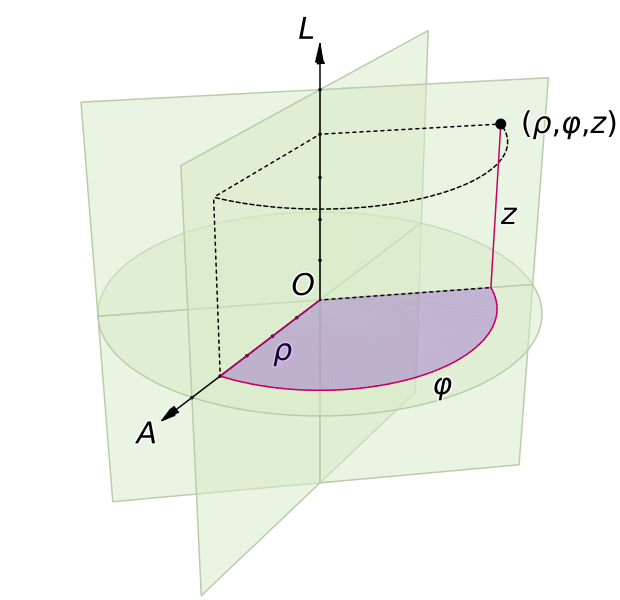
\includegraphics[width=0.8\linewidth]{fig/620px-Coord_system_CY.png}}

\vspace{6mm}



Koordinatytorna för $\rho, \phi, z$ är då en cylinder med $z$-axeln som symmetriaxel och med radien $\rho$, ett plan som utgår från $z$-axeln och bildar en vinkel $\phi$ med $x$-axeln, samt ett plan parallellt med $xy$-planet och med $z$-koordinaten $z$. 



\vspace{6mm}

% inline figure
\centerline{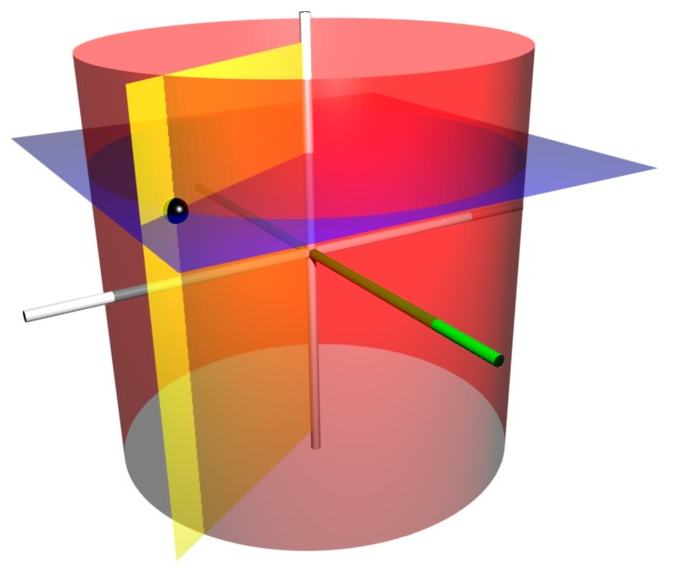
\includegraphics[width=0.8\linewidth]{fig/Cylindrical_coordinate_surfaces.png}}

\vspace{6mm}



Koordinatlinjerna för $\rho, \phi, z$ blir då en stråle som utgår från $z$-axeln och bildar vinkeln $\phi$ med $x$-axeln, en cirkel med radien $\rho$ och en linje parallell med $z$-axeln.
\end{notice_mdfboxadmon} % title: Exempel: cylindriska koordinater



\subsection{Enhetsvektorer}
Om vi nu studerar en liten förskjutning av ortsvektorn, $\mbox{d}\vec{r}$, så kan vi i och med att ortsvektorn är en funktion av $u_1, u_2, u_3$ skriva denna som 
\begin{equation}
  \mbox{d}\vec{r} = \frac{\partial \vec{r}}{\partial u_1} \mbox{d}u_1 +
\frac{\partial \vec{r}}{\partial u_2} \mbox{d}u_2 + 
\frac{\partial \vec{r}}{\partial u_3} \mbox{d}u_3.
\label{eq:forskjutningsvektor}
\end{equation}

Tänk nu på att den partiella derivatan $\partial \vec{r}/\partial u_1$
är definierad som derivatan då vi håller $u_2$ och $u_3$ fixa.
Därför måste $\partial \vec{r}/\partial u_1$ vara en tangentvektor
till koordinatkurvan för $u_1$.  Vi kan då definiera en enhetsvektor 
för $u_1$ som
\begin{equation}
  \hat{e}_1 = \frac{1}{h_1} \frac{\partial \vec{r}}{\partial u_1},
\end{equation}
där 
\begin{equation}
  h_1 = \left|\frac{\partial \vec{r}}{\partial u_1}\right|
\end{equation}
kallas för skalfaktorn.  På samma sätt kan vi bestämma skalfaktorer och enhetsvektorer till $u_2$ och $u_3$. Förskjutningsvektorn $\mbox{d}\vec{r}$ kan vi nu skriva som
\begin{equation}
  \mbox{d}\vec{r} = h_1\hat{e}_1 \mbox{d}u_1 + h_2\hat{e}_2\mbox{d}u_2 +
h_3\hat{e}_3\mbox{d}u_3.
\label{eq:forskjutningsvektor_skalfaktor}
\end{equation}

\paragraph{Alternativ definition.}
Ett alternativ till att använda de normerade tangentvektorerna som enhetsvektorer är att använda normalvektorerna till koordinatytorna. Betrakta t.ex.
\begin{equation}
u_1 = u_1(x,y,z) = \mathrm{konstant}.
\end{equation}
Detta motsvarar en nivåyta till ett skalärfält. Normalvektorn ges alltså av $\vnabla u_1$.
Det gäller alltid att 
\begin{equation}
\vnabla u_i \cdot \frac{\partial \vec{r}}{\partial u_j} = \delta_{ij}.
\end{equation}
När vi inskränker oss till ortogonala system gäller dessutom att $\vnabla u_i \parallel \frac{\partial \vec{r}}{\partial u_i}$. Notera dock att dessa vektorer i allmänhet kan ha \emph{olika} längd. Faktum är att följande samband gäller för ortogonala system
\begin{equation}
\hat{e}_i 
= \frac{1}{h_i} \frac{\partial \vec{r}}{\partial u_i}
= h_i \vnabla u_i.
\end{equation}


\begin{notice_mdfboxadmon}[Exempel: Enhetsvektorer för cylindriska koordinater]
I cylindriska koordinater är $\vec{r} = (\rho\cos \phi, \rho\sin \phi, z)$.  Vi kan då beräkna
\begin{align}
  \frac{\partial \vec{r}}{\partial \rho} &= \left(\cos \phi, \sin \phi, 0\right), \\ 
  \frac{\partial \vec{r}}{\partial \phi} &= \left(-\rho \sin\phi, \rho \cos \phi,
0\right), \\ 
  \frac{\partial \vec{r}}{\partial z} &= \left(0,0,1\right).
\end{align}
Skalfaktorerna blir då
\begin{align}
  h_\rho &= \left(\cos^2\phi + \sin^2\phi\right)^{1/2} = 1, \\ 
  h_\phi &= \left(\rho^2 \cos^2\phi + \rho^2 \sin^2\phi\right)^{1/2} = \rho, \\ 
  h_z &= 1.
\end{align}
Enhetsvektorerna blir
\begin{align}
  \hat{\rho} &= \left(\cos\phi, \sin\phi,0\right), \\ 
  \hat{\phi} &= \left(-\sin\phi, \cos\phi,0\right), \\ 
  \hat{z} &= \left(0,0,1\right).
\end{align}
Förskjutningsvektorn kan då skrivas som
\begin{equation}
  \mbox{d}\vec{r} = \hat{\rho} \mbox{d}\rho + \rho \hat{\phi} \mbox{d} \phi + \hat{z} \mbox{d}z.
\end{equation}
\end{notice_mdfboxadmon} % title: Exempel: Enhetsvektorer för cylindriska koordinater



I fortsättningen skall vi begränsa oss till koordinatsystem med ortogonala enhetsvektorer, dvs
\begin{equation}
\hat{e}_i \cdot \hat{e}_j = \delta_{ij} = \left\{
\begin{array}{ll}
1 & \,\mbox{om}\,\, i = j \\ 
0 & \,\mbox{annars}\\ 
\end{array}\right.
\end{equation}
där vi passat på att introducera Kroneckers delta, $\delta_{ij}$.

Vi skall också anta att enhetsvektorerna bildar ett högersystem
\begin{equation}
\hat{e}_1 \times \hat{e}_2 = \hat{e}_3
\end{equation}

\emph{Visa att enhetsvektorerna i de cylindriska koordinaterna uppfyller dessa villkor.}

Vi kan nu härleda några användbara samband som båglängden längs en kurva
\begin{equation}
\mbox{d}s^2 = \mbox{d}\vec{r}\cdot \mbox{d}\vec{r} = h_1^2\mbox{d}u_1^2 + h_2^2
\mbox{d}u_2^2 + h_3^2 \mbox{d}u_3^2.
\end{equation}
Betrakta ovanstående båglängd för fallet då $du_2=du_3=0$. Det står då klart att vi kan tolka $h_1 du_1$ som båglängden $ds_1$, dvs som en infinitesimal förflyttning i $u_1$-riktningen. Notera därför att $h_i du_i$ alltid måste ha enheten längd.

Ett ytelement $\mbox{d}\vec{S}_1$ på koordinatytan $u_1$ är en rektangel som  genereras av $\mbox{d}u_2$ och $\mbox{d}u_3$. Rektangelns sidor har då längderna $h_2\mbox{d}u_2$ och $h_3\mbox{d}u_3$.  Ytelementet blir
\begin{equation}
  \mbox{d}\vec{S}_1 =  \hat{e}_1 h_2 h_3 \mbox{d}u_2 \mbox{d}u_3,
\end{equation}
och på samma sätt kan vi beräkna ytelementen på koordinatytorna för $u_2$ och $u_3$.  

Analogt kan vi beräkna volymelementet som genereras av  $\mbox{d}u_1$, $\mbox{d}u_2$ och $\mbox{d}u_3$, vilket blir
\begin{equation}
  \mbox{d}V = h_1 h_2 h_3 \mbox{d}u_1 \mbox{d}u_2 \mbox{d}u_3.
\end{equation}


\begin{notice_mdfboxadmon}[Exempel: båg- yt- och volymselement i cylindriska koordinater]
Bågelementet i cylindriska koordinater blir
\begin{equation}
  \mbox{d}s^2 = \mbox{d}\rho^2 + \rho^2\mbox{d}\theta^2 + \mbox{d}z^2.
\end{equation}
Ett ytelement på $\rho$-ytan skrives
\begin{equation}
  \mbox{d}\vec{S}_\rho = \hat{e}_\rho \rho \mbox{d}\phi\mbox{d}z,
\end{equation}
på $\phi$-ytan
\begin{equation}
  \mbox{d}\vec{S}_\phi = \hat{e}_\phi \mbox{d}\rho\mbox{z}
\end{equation}
och på $z$-ytan
\begin{equation}
  \mbox{d}\vec{S}_z = \hat{e}_z \rho\mbox{d}\rho \mbox{d}\phi.
\end{equation}
Volymelementet kan vi skriva som
\begin{equation}
  \mbox{d}V = \rho\mbox{d}\rho \mbox{d}\phi\mbox{d}z.
\end{equation}
\end{notice_mdfboxadmon} % title: Exempel: båg- yt- och volymselement i cylindriska koordinater



\subsection{Vektoroperatorer i kroklinjiga koordinater}

\paragraph{Gradient.}
Betrakta ett skalärt fält $\phi$.  Om vi förflyttar oss en sträcka $\mbox{d}\vec{r}$ så förändras $\phi$ 
\begin{equation}
  \mbox{d}\phi = \vnabla \phi \cdot \mbox{d}\vec{r}.
\end{equation}
Samtidigt, om vi skriver $\phi$ som en funktion av $u_1, u_2$ och $u_3$ får vi
\begin{align}
  \mbox{d}\phi &= \frac{\partial \phi}{\partial u_1}\mbox{d}u_1 + 
\frac{\partial \phi}{\partial u_2}\mbox{d}u_2 +
\frac{\partial \phi}{\partial u_3}\mbox{d}u_3 =
\frac{1}{h_1} \frac{\partial \phi}{\partial u_1} h_1 \mbox{d}u_1 +
\frac{1}{h_2} \frac{\partial \phi}{\partial u_2} h_2 \mbox{d}u_2 +
\frac{1}{h_3} \frac{\partial \phi}{\partial u_3} h_3 \mbox{d}u_3 \nonumber \\ 
 &=
\left(\frac{1}{h_1} \frac{\partial \phi}{\partial u_1} \hat{e}_1 +
\frac{1}{h_2} \frac{\partial \phi}{\partial u_2} \hat{e}_2 +
\frac{1}{h_3} \frac{\partial \phi}{\partial u_3} \hat{e}_3\right) \cdot 
\mbox{d}\vec{r}
\end{align}
Förflyttningen $\mbox{d}\vec{r}$ (ovan) kan vi i de nya koordinaterna skriva som [se ekv. (\ref{eq:forskjutningsvektor_skalfaktor})]
\begin{equation}
  \mbox{d}\vec{r} = h_1 \hat{e}_1 \mbox{d}u_1 + h_2 \hat{e}_2 \mbox{d}u_2
+ h_3 \hat{e}_3 \mbox{d}u_3.
\end{equation}
Då kan vi identifiera uttrycket inom parentesen som gradienten i de nya koordinaterna $u_1, u_2, u_3$
\begin{equation}
  \vnabla \phi = \frac{1}{h_1} \frac{\partial \phi}{\partial u_1} \hat{e}_1
+ \frac{1}{h_2}
\frac{\partial \phi}{\partial u_2} \hat{e}_2 
+ \frac{1}{h_3} \frac{\partial \phi}{\partial u_3} \hat{e}_3.
\end{equation}

\paragraph{Gradient i cylindriska koordinater:}
I cylindriska koordinater blir gradienten
\begin{equation}
  \vnabla f = \frac{\partial f}{\partial \rho} \hat{\rho} + \frac{1}{\rho}
\frac{\partial f}{\partial \phi} \hat{\phi} + \frac{\partial f}{\partial z} \hat{z}.
\end{equation}


\begin{notice_mdfboxadmon}[Exempel: skalärfält och dess gradient i olika koordinatsystem]
Ett skalärfält är givet i Cartesiska koordinater
\begin{equation}
\beta = x^2 + y^2.
\end{equation}
Motsvarande skalärfält i plana polärkoordinater blir
\begin{equation}
\beta = r^2\cos^2\theta + r^2 \sin^2\theta = r^2.
\end{equation}
Gradienten i Cartesiska koordinater blir
\begin{equation}
\vnabla \beta = \hat{x} \partial_x \beta + \hat{y} \partial_y \beta = 2 (x \hat{x} + y \hat{y}).
\end{equation}
Medan i plana polärkoordinater blir den
\begin{equation}
\vnabla \beta = \hat{e}_r \partial_r + \hat{e}_\theta \frac{1}{r} \partial_\theta \beta = 2 r \hat{e}_r.
\end{equation}
Eftersom $x \hat{x} + y \hat{y} = r \hat{e}_r$ är det uppenbart att detta är samma vektor!
\end{notice_mdfboxadmon} % title: Exempel: skalärfält och dess gradient i olika koordinatsystem




\begin{notice_mdfboxadmon}[Exempel: Tentauppgift 2010-08-26: 1b]
För vilka värden på $\alpha,\beta,\gamma$ har det tvådimensionella koordinatsystemet med koordinater $\xi$ och $\eta$, givna av
\begin{align}
\xi &= x^2 - y^2 \\ 
\eta &= \alpha x^2 + \beta x y + \gamma y^2
\end{align}
ortogonala basvektorer?

\paragraph{Lösning.}
Vi kan konstruera basvektorer på två sätt:
\begin{itemize}
\item $\hat{e}_i \propto \frac{\partial \vec{r}}{\partial u_i}$

\item $\hat{e}_i \propto \vnabla u_i$
\end{itemize}

\noindent
Det första sättet innebär att vi behöver räkna ut storheterna $\frac{\partial x}{\partial u_i}$ och $\frac{\partial y}{\partial u_i}$, dvs vi behöver veta $x=x(\xi,\eta),\; y=y(\xi,\eta)$. Vi skulle behöva invertera det givna koordinatsambandet.

Det andra sättet kräver istället $\frac{\partial \xi}{\partial x}$ och $\frac{\partial \xi}{\partial y}$ (samt motsvarande för $\eta$) och detta blir enkelt med de givna koordinattransformationerna. Vi får
\begin{align}
\vnabla \xi &= 2x \hat{x} - 2y \hat{y} \\ 
\vnabla \eta &= (2 \alpha x + \beta y)\hat{x} + (\beta x + 2 \gamma y) \hat{y}
\end{align}
För att koordinatsystemet skall vara ortogonalt behöver vi
\begin{equation}
\hat{e}_\xi \cdot \hat{e}_\eta = 0 \qquad \Rightarrow \qquad \vnabla \xi \cdot \vnabla \eta=0.
\end{equation}
Från uttrycken för dessa gradienter ovan får vi
\begin{equation}
\vnabla \xi \cdot \vnabla \eta = 2x (2 \alpha x + \beta y) - 2 y (\beta x + 2 \gamma y) 
= 4 \alpha x^2 - 4 \gamma y^2.
\end{equation}
För att få $\vnabla \xi \cdot \vnabla \eta=0$ måste vi ha $\alpha = \gamma = 0$, medan $\beta$ är godtyckligt.




\vspace{6mm}

% inline figure
\centerline{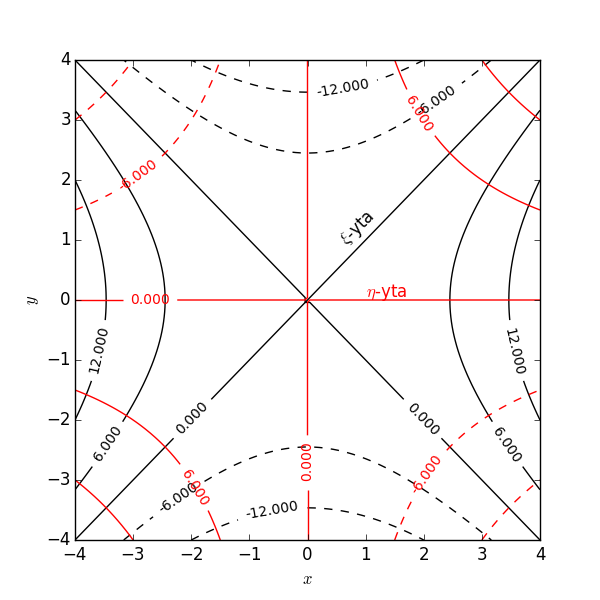
\includegraphics[width=0.8\linewidth]{fig/koordinatytor.png}}

\vspace{6mm}
\end{notice_mdfboxadmon} % title: Exempel: Tentauppgift 2010-08-26: 1b



Mer text...


\begin{notice_mdfboxadmon}[Exempel: Fältlinjer i kroklinjiga koordinater]
Låt oss konstruera och rita fältlinjerna till en så kallad virveltråd
\begin{equation}
\vec F = \frac{J}{2\pi\rho} \hat{\varphi}, 
\end{equation}
som alltså är uttryckt i cylindriska koordinater. Notera att detta fält är singulärt längs hela $z$-axeln vid $\rho=0$, men vi kommer här enbart att betrakta $\rho > 0$.

\paragraph{Lösning.}
Vi kan rita fältlinjerna på två sätt:
\begin{itemize}
\item Det första alternativet är förstås att finna ett explicit uttryck för fältlinjerna genom att lösa de definierande differentialekvationerna. Sedan kan vi definiera dessa kurvor som en funktion i Matlab (eller Python) och rita upp den explicit för några olika startpunkter.

\item Det andra alternativt är att utnyttja funktionen 'streamline' i Matlab ('streamplot i Python) och mata in vektorfältet på ett grid av olika koordinatpunkter. Notera dock att detta alternativ bygger på att vi transformerar till ett Cartesiskt koordinatsystem.
\end{itemize}

\noindent
\bpypro
### Start initialization
import sys
import numpy as np
import matplotlib.pyplot as plt
### End initialization
### Start Alt. 2: Streamlines with streamplot ###
w = 3
Y, X = np.mgrid[-w:w:100j, -w:w:100j]
R = np.sqrt(X**2+Y**2)
U = -Y / R**2 # Note that -Y/R = -sin(phi)
V = X / R**2  # Note that X/R = cos(phi)

fig = plt.figure()
ax = fig.add_subplot(111)

strm = ax.streamplot(X, Y, U, V, linewidth=2)

ax.set_title(r'Streamplot, vortex field $\vec{F} = \frac{J}{2\pi\rho}\hat\varphi$')
ax.set_xlabel('$x$')
ax.set_ylabel('$y$')

ax.set_aspect('equal')

plt.savefig('streamlines-vortex.png')
### End Alt. 2

### Start Alt. 1: Streamlines as 2d curves ###
def curve(rho0,x):
    """Fieldline for vortex streamlines in Cartesian coordinates.
    Assume z=0 => Fieldline in xy-plane.
    We also avoid the singularity at x=y=0."""
    if max(abs(x)) > rho0:
        print('Fieldline for rho_0=%3.1f is only defined for |x| <= %3.1f' %(rho0,rho0))
        return None
    return np.sqrt(rho0**2 - x**2)

fig = plt.figure()
ax = fig.add_subplot(111)

# Grid of x points
nx = 64

# Streamline constant
for rho0 in np.linspace(1,3,5):

    # Grid of x points
    x = np.linspace(-rho0,rho0, nx)

    yp = curve(rho0,x)
    ym = -curve(rho0,x)

    # Plot the streamlines with an appropriate colormap and arrow style
    ax.plot(x, yp, 'b-', x, ym, 'b-', linewidth=2)
    ax.annotate("", xy=(max(x), 0.1), xytext=(max(x), 0), arrowprops=dict(arrowstyle="->",color='b'))

ax.set_title(r'Streamplot, vortex field $\vec{F} = \frac{J}{2\pi\rho}\hat\varphi$')
ax.set_xlabel('$x$')
ax.set_ylabel('$y$')

ax.set_aspect('equal')
### End Alt. 1

#plt.show()
plt.savefig('streamlines-vortex-curves.png')
\epypro




\vspace{6mm}

% inline figure
\centerline{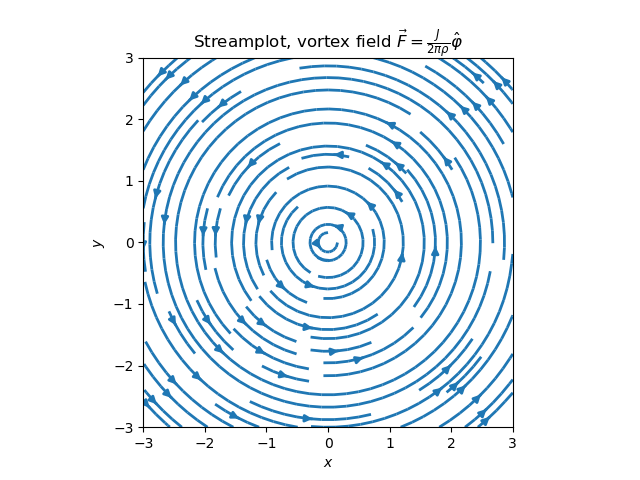
\includegraphics[width=0.8\linewidth]{fig/streamlines-vortex.png}}

\vspace{6mm}
\end{notice_mdfboxadmon} % title: Exempel: Fältlinjer i kroklinjiga koordinater



% ------------------- end of main content ---------------

% #ifdef PREAMBLE
\end{document}
% #endif

